\documentclass[aspectratio=169]{beamer}
\usepackage{lphs}

\SetupImages{L2-Images/}{jpg}
\newcommand{\firstcircle}{(-1,0) circle (1.5)}
\newcommand{\secondcircle}{(1,0) circle (1.5)}
\newcommand{\thirdcircle}{(0,1.73) circle (1.5)}

\begin{document}

\section{Силлогизмы}

\begin{frame}
\begin{columns}
\column{0.4\textwidth}
\begin{center}
\begin{Reason}
	\from{Все люди смертны}
	\from{Сократ -- человек}
	\conc{Сократ -- смертен}
\end{Reason}
\end{center}

\column{0.6\textwidth}
\begin{center}
\begin{tikzpicture}[x=1.3cm,y=-1.3cm]
\uncover<3->{
	\begin{scope}[even odd rule]% first circle without the second
	\clip \secondcircle (-2.5,-1.5) rectangle (2.5,1.5);
	\fill[gray] \firstcircle;
	\end{scope}}
\uncover<4->{
	\node at (0,0) {Сократ};	
}
\uncover<2->{
	\draw \firstcircle node[left] {Люди};
	\draw \secondcircle node[right] {Смертны};
}
\end{tikzpicture}
\end{center}
\end{columns}
\end{frame}

\begin{frame}
	\begin{columns}
		\column{0.4\textwidth}
		\begin{center}
			\begin{Reason}
				\from{Все $A$ есть $B$}
				\from{Некоторый $X$ есть $A$}
				\conc{$X$ есть $B$}
			\end{Reason}
		\end{center}
		
		\column{0.6\textwidth}
		\begin{center}
			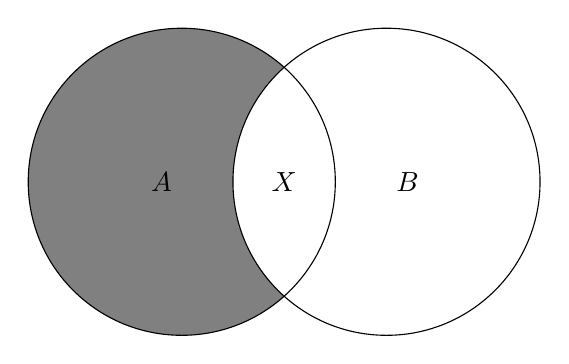
\begin{tikzpicture}[x=1.3cm,y=-1.3cm]
		
				\begin{scope}[even odd rule]% first circle without the second
				\clip \secondcircle (-2.5,-1.5) rectangle (2.5,1.5);
				\fill[gray] \firstcircle;
				\end{scope}
			
				\node at (0,0) {$X$};	
			
				\draw \firstcircle node[left] {$A$};
				\draw \secondcircle node[right] {$B$};
			\end{tikzpicture}
		\end{center}
	\end{columns}
\end{frame}

\begin{frame}
\begin{columns}
\column{0.4\textwidth}
\begin{center}
\begin{Reason}
	\from{Все кошачьи хищники}
	\from{Все львы кошачьи}
	\conc{Все львы хищники}
\end{Reason}
\end{center}
\column{0.6\textwidth}
\begin{center}
\begin{tikzpicture}[x=1.3cm,y=-1.3cm]

\uncover<3->{\begin{scope}[even odd rule]% first circle without the second
\clip \secondcircle (-2.5,-1.5) rectangle (2.5,3.25);
\fill[gray] \firstcircle;
\end{scope}}

\uncover<4->{\begin{scope}[even odd rule]% first circle without the second
\clip \firstcircle (-2.5,-1.5) rectangle (2.5,3.25);
\fill[gray] \thirdcircle;
\end{scope}}

\uncover<2->{\draw \firstcircle node {К};
\draw \secondcircle node {Х};
\draw \thirdcircle node {Л};
}
\end{tikzpicture}
\end{center}
\end{columns}
\end{frame}

\begin{frame}
	\begin{columns}
		\column{0.5\textwidth}
		\begin{center}
			\begin{Reason}
				\from{Некоторые небольшие птицы питаются медом}
				\from{Все питающиеся медом птицы цветные}
				\conc{Некоторые цветные птицы небольшие}
			\end{Reason}
		\end{center}
		\column{0.5\textwidth}
		\begin{center}
			\begin{tikzpicture}[x=1cm,y=-1cm]
			
			\uncover<3->{\begin{scope}
				\clip \secondcircle;
				\fill[red] \firstcircle;
				\end{scope}}
			
			\uncover<4->{\begin{scope}[even odd rule]% first circle without the second
				\clip \thirdcircle (-2.5,-1.5) rectangle (2.5,3.25);
				\fill[gray] \secondcircle;
				\end{scope}}
			
			\uncover<2->{\draw \firstcircle node {Н};
				\draw \secondcircle node {М};
				\draw \thirdcircle node {Ц};
			}
			\end{tikzpicture}
		\end{center}
	\end{columns}
\end{frame}



\begin{frame}
	\begin{columns}
		\column{0.5\textwidth}
		\begin{center}
			\begin{Reason}
				\from{Все яркие цветы ароматны}
				\from{Ни один ароматный цветок не выращен  в помещении}
				\conc{Ни один выращенный в помещении цветок не ярок}
			\end{Reason}
		\end{center}
		\column{0.5\textwidth}
		\begin{center}
			\begin{tikzpicture}[x=1cm,y=-1cm]
			
			\uncover<3->{\begin{scope}[even odd rule]% first circle without the second
				\clip \secondcircle (-2.5,-1.5) rectangle (2.5,3.25);
				\fill[gray] \firstcircle;
				\end{scope}}
			
			\uncover<4->{\begin{scope}
				\clip \thirdcircle;
				\fill[gray] \secondcircle;
				\end{scope}}
			
			\uncover<2->{\draw \firstcircle node {Я};
				\draw \secondcircle node {А};
				\draw \thirdcircle node {П};
			}
			\end{tikzpicture}
		\end{center}
	\end{columns}
\end{frame}

\begin{frame}
	\begin{columns}
		\column{0.4\textwidth}
		\begin{center}
			\begin{Reason}
				\from{Все птицы кладут яйца}
				\from{Крокодил кладет яйца}
				\conc{Крокодил -- это птица}
			\end{Reason}
		\end{center}
		
		\column{0.6\textwidth}
		\begin{center}
			\begin{tikzpicture}[x=1.3cm,y=-1.3cm]
			\uncover<3->{
				\begin{scope}[even odd rule]% first circle without the second
				\clip \secondcircle (-2.5,-1.5) rectangle (2.5,1.5);
				\fill[gray] \firstcircle;
				\end{scope}}
			\uncover<4->{
				\node at (0.3,0) {Крокодил};	
			}
			\uncover<2->{
				\draw \firstcircle node[left] {П};
				\draw \secondcircle node[right] {Я};
			}
			\end{tikzpicture}
		\end{center}
	\end{columns}
\end{frame}

\begin{frame}
	\begin{columns}
		\column{0.5\textwidth}
		\begin{center}
			\begin{Reason}
				\from{Все волки -- хищники}
				\from{Все львы -- хищники}
				\conc{Все волки -- львы}
			\end{Reason}
		\end{center}
		\column{0.5\textwidth}
		\begin{center}
			\begin{tikzpicture}[x=1cm,y=-1cm]
			
			\uncover<3->{\begin{scope}[even odd rule]
				\clip \thirdcircle (-2.5,-1.5) rectangle (2.5,3.25);
				\fill[gray] \firstcircle;
				\end{scope}}
			
			\uncover<4->{\begin{scope}[even odd rule]
				\clip \thirdcircle (-2.5,-1.5) rectangle (2.5,3.25);
				\fill[gray] \secondcircle;
				\end{scope}}
			
			\uncover<2->{\draw \firstcircle node {В};
				\draw \secondcircle node {Л};
				\draw \thirdcircle node {Х};
			}
			\end{tikzpicture}
		\end{center}
	\end{columns}
\end{frame}

\section{Валидность суждений}

\section{Обоснованность суждений}

\begin{frame}
\begin{minipage}[center]{0.6\textwidth}
\begin{Reason}
\from{Все металлы проводят электрический ток}
\from{Ртуть -- металл}
\conc{Ртуть проводит электрический ток}
\end{Reason}
\end{minipage}
\end{frame}

\begin{Person}{Witgenstein}{Людвиг Витгенштейн}{1889--1951}
\Citation{
Мир состоит из фактов, а не вещей.\\[1cm]

Слова соединяются между собой также, как соединяются факты, образуя с ними зеркальную пару.
}{
Логико-философский трактат, 1921 г.
}

\end{Person}

\section{Модальные логики?}



\end{document}